\subsubsection{UC26 - Daily Rewards}
\begin{itemize}
	\item \textbf{Attori Primari}: utente autenticato;
	\item \textbf{Descrizione}: l'applicazione rende disponibile una tabella che illustra i premi giornalieri del mese corrente. La tabella è organizzata sotto forma di calendario, in cui associa a quasi ogni giorno del mese corrente un premio. Ogni giorno del mese ha un premio riscattabile solo se si ha riscattato il premio del giorno precedente altrimenti rimarrà impostato il premio non ritirato. L'avanzamento da un premio all'altro è previsto solo in caso di ritiro del premio precedente. 
	Sotto alla tabella è presente un bottone "Ritira premio" che si disattiva dopo il primo utilizzo fino alla mezzanotte del giorno corrente.\\
	I premi ottenibili possono includere:
	\begin{itemize}
		\item sconti su e-commerce o buoni spesa;
		\item sconto sul prossimo viaggio con \textit{GaiaGo};
		\item viaggio gratuito con \textit{GaiaGo};
		\item accessori per l'auto del minigioco;
		\item bonus di punti esperienza;
		\item oggetti virtuali esclusivi per il minigioco.
	\end{itemize}
	\item \textbf{Scenario principale}: l'utente preme il pulsante relativo alla tabella dei Daily Rewards da cui può visualizzare i premi disponibili per il mese corrente e decidere di ritirare il corrispettivo premio [UC27].
	Ogni premio può essere ritirato solo una volta;
	\item \textbf{Estensioni}: 
		\begin{itemize}
			\item ritiro del premio giornaliero [UC26].
		\end{itemize}
	\item \textbf{Precondizione}: l'utente ha premuto il pulsante Daily Rewards;
	\item \textbf{Postcondizione}: l'utente ha visualizzato i premi disponibili per il mese corrente e può aver ritirato il premio corrispettivo se non lo ha precedentemente fatto [UC27]. 
\end{itemize} 
\begin{figure}[h]
	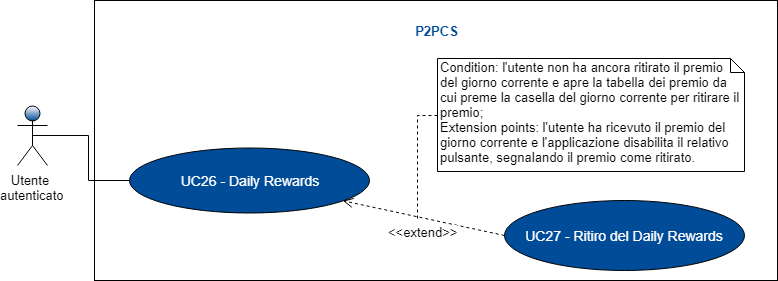
\includegraphics[width=13.2cm]{res/images/UC24Daily.png}
	\centering
	\caption{UC26 - Daily Rewards}
\end{figure}
\subsubsection{UC27 - Ritiro del Daily Rewards}
\begin{itemize}
	\item \textbf{Attori Primari}: utente autenticato;
	\item \textbf{Descrizione}: l'applicazione rende disponibile dei premi giornalieri, illustrati e con la possibilità di ritirarli tramite l'apposito pulsante di raccoglimento premi (una sola volta);
	\item \textbf{Scenario principale}: l'utente sta visualizzando la tabella dei premi giornalieri e preme il pulsante "Ritira premio" per ritirarlo;
	\item \textbf{Precondizione}: l'utente apre la tabella dei premi e preme il pulsante "Ritira premio" per ritirare il premio;
	\item \textbf{Postcondizione}: l'utente riceve il premio se non lo ha già ritirato precedentemente e l'applicazione disabilita il relativo pulsante mostrando, tramite un pop-up, il relativo premio.  
\end{itemize} 